\documentclass{article}
\usepackage[
paperwidth = 100mm, 
paperheight =80mm, 
textwidth = 100mm,
textheight = 80mm,
nohead,
nofoot,
nomarginpar]{geometry}
\usepackage{amsmath,amsfonts,amssymb}
\usepackage{tikz,pgfplots}
\usetikzlibrary{arrows,arrows.meta,bending,calc,decorations,shadings,shadows,shapes,shapes.arrows,shapes.geometric}
\usetikzlibrary{calc,fadings,decorations.pathreplacing}
\usepgfplotslibrary{units,fillbetween,groupplots,colorbrewer}
\usetikzlibrary{pgfplots.colorbrewer,}
\usepackage{pgfplotstable}
\usetikzlibrary{3d,spy}
\usepgfmodule{plot}
\usepackage{scalerel}
\usepackage{graphicx}
\usepackage{epstopdf}
\epstopdfsetup{outdir=out-ruco/,suffix=-generated}
\newcommand*{\xMin}{-1}%
\newcommand*{\xMax}{10}%
\newcommand*{\yMin}{-5}%
\newcommand*{\yMax}{5}%

\definecolor{As}{RGB}{255,255,0}
\definecolor{Al}{RGB}{173,216,230}
\definecolor{Ga}{RGB}{0,128,150}
\begin{document}
	\thispagestyle{empty}
\begin{tikzpicture}[remember picture,overlay]
\draw[step=.5cm,gray,very thin,opacity=0.2] (0,0) grid(\xMax,\yMax);
\foreach \i in {\xMin,...,\xMax} {
\draw [very thin,gray,opacity=0.2] (\i,\yMin) -- (\i,\yMax)  node [below,opacity=1] at (\i,\yMin) {$\i$};
}
\foreach \i in {\yMin,...,\yMax} {
\draw [very thin,gray,opacity=0.2] (\xMin,\i) -- (\xMax,\i) node [left,opacity=1] at (\xMin,\i) {$\i$};
}
							
\node[anchor=center](s1) at (current page.center){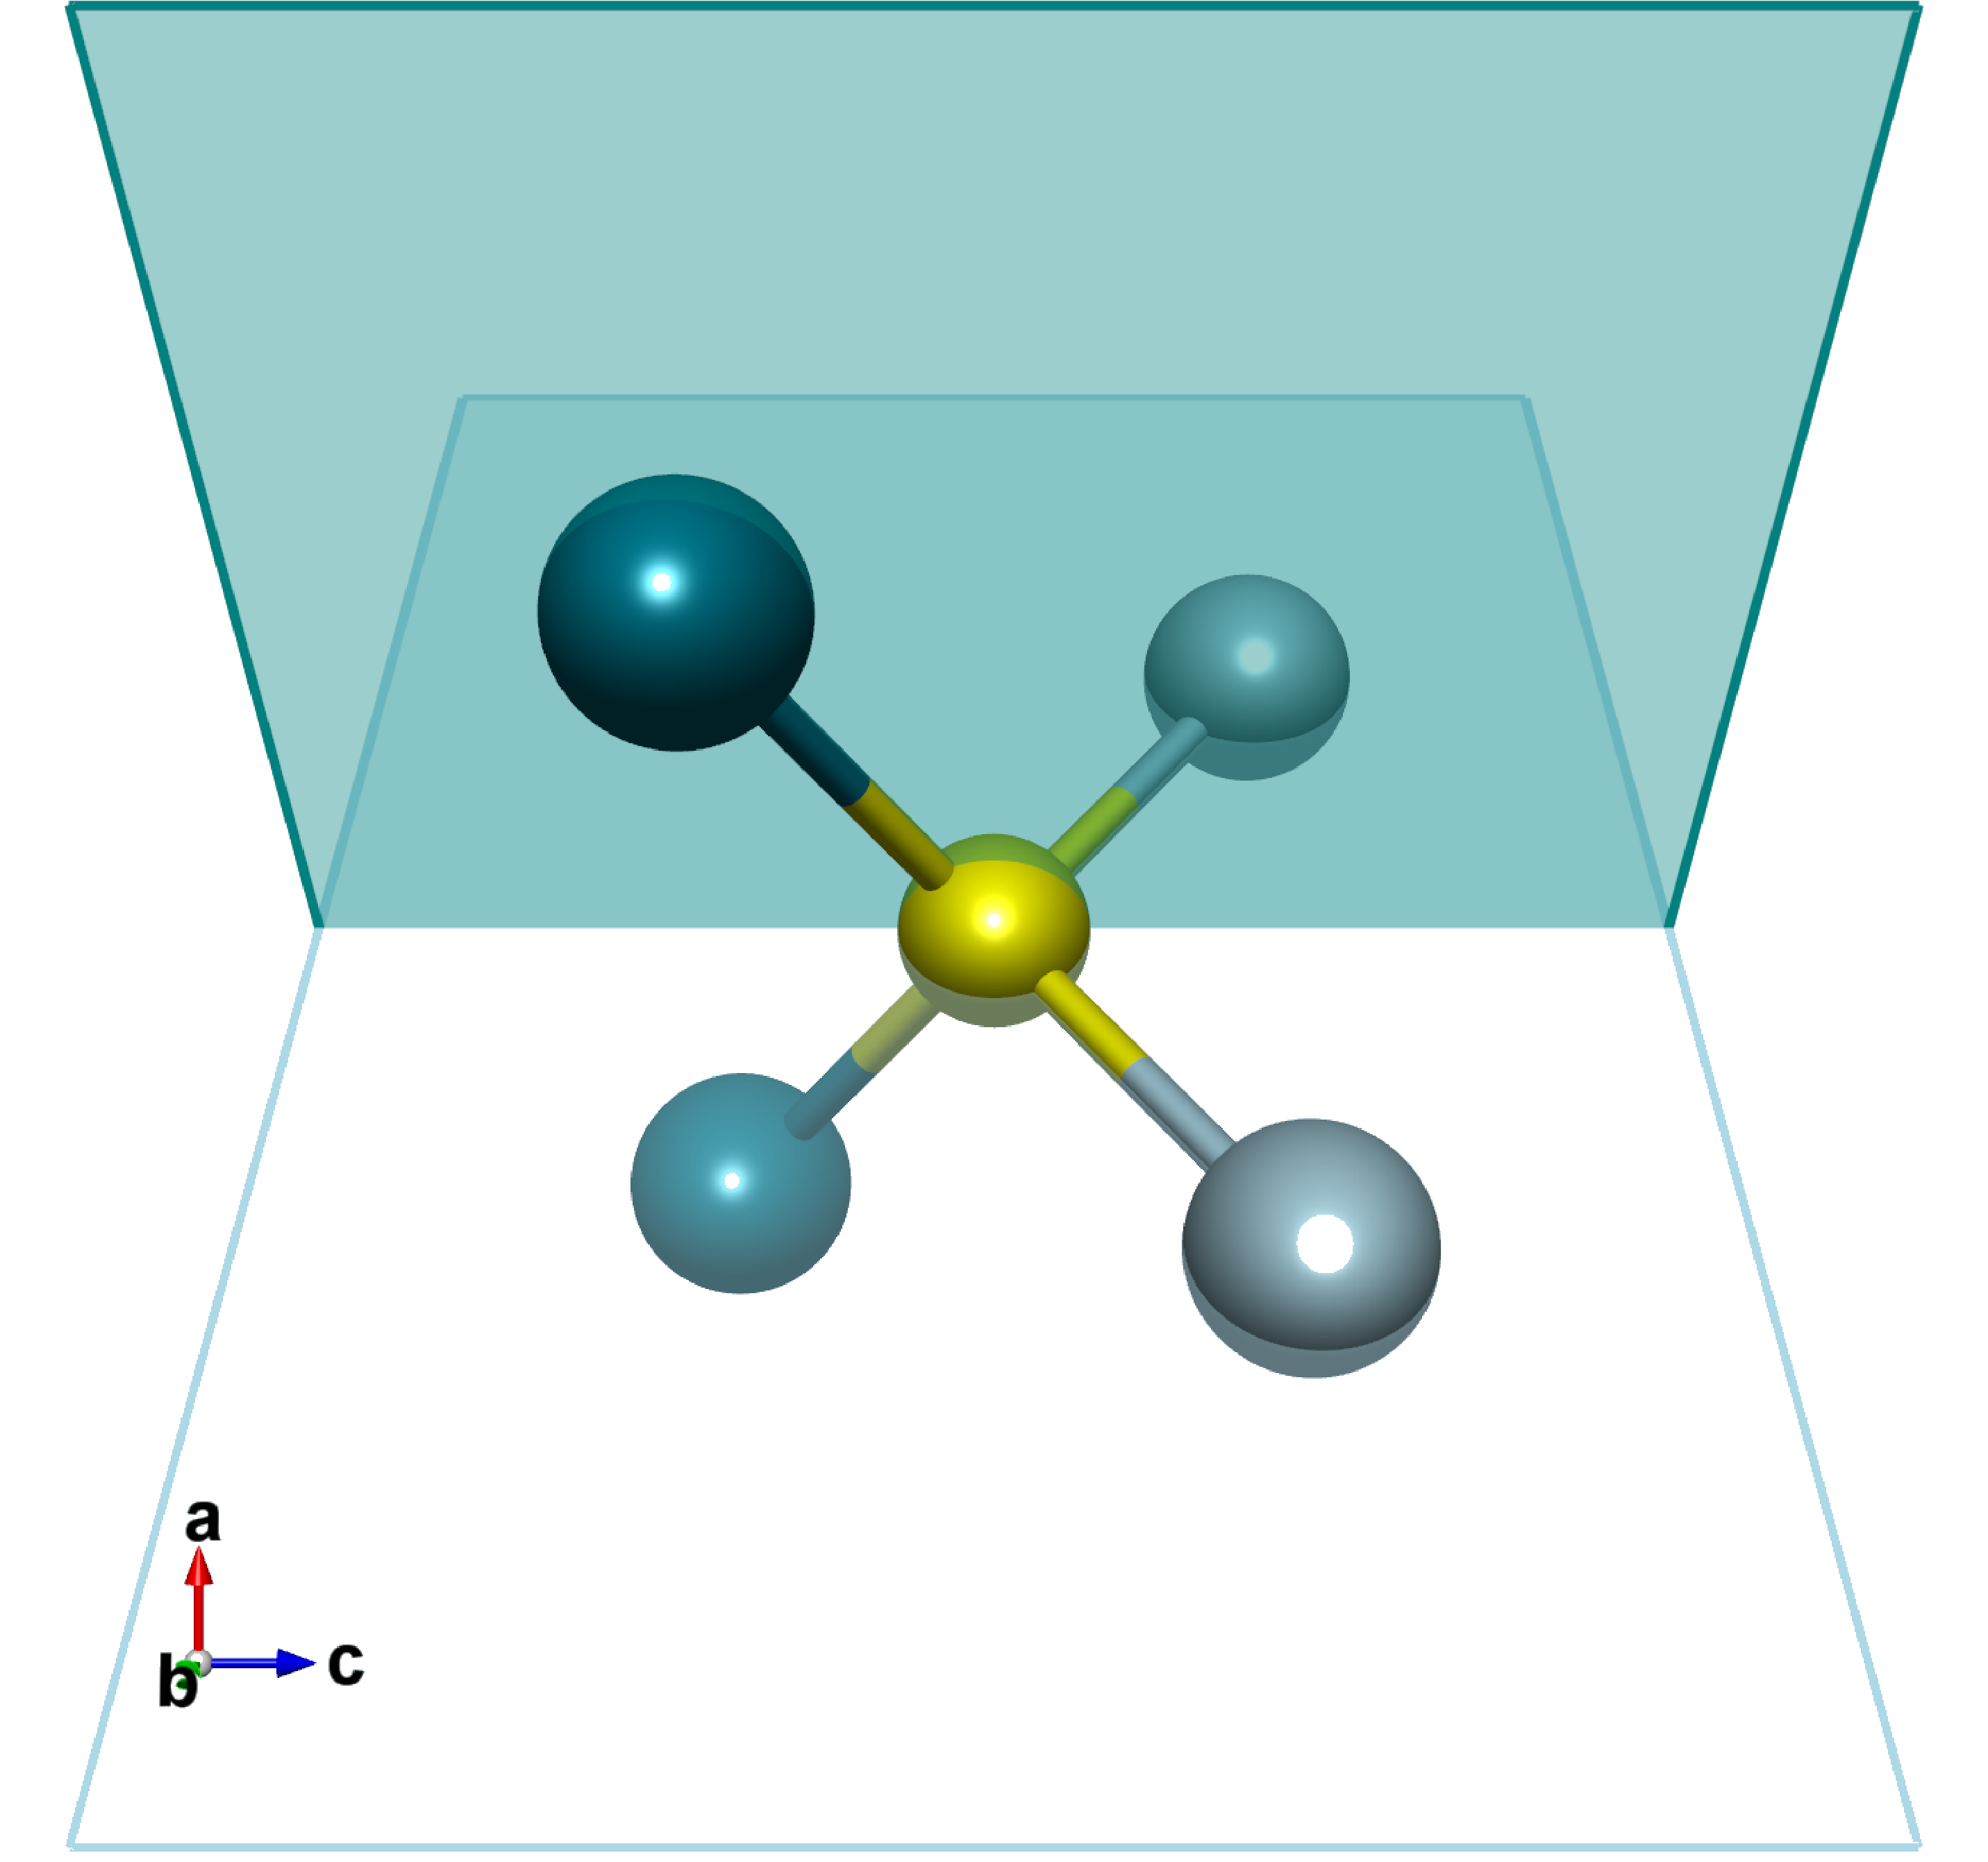
\includegraphics[width=\textwidth]{/media/labfiles/ruco/phd-ssp/phd-codes/atom-structures/symmetry3-algaas}};

\node[scale=2,rotate=0,font=\boldmath] 
	at ([xshift=-1.9cm,yshift=3.2cm]s1.center)
		{\(\left[110\right]\)};
\node[scale=2,rotate=7,font=\boldmath] 
	at ([xshift=3.7cm,yshift=3.3cm]s1.center)
		{$\left[1\overline{1}0\right]$};

\shade [ball color=Ga] ([xshift=5mm,yshift=7mm]s1.west) circle (0.35) node[label=right:{\Large\, Ga}] { } ;
\shade [ball color=Al] ([xshift=5mm,yshift=16mm]s1.west) circle (0.33) node[label=right:{\Large\, Al}] { } ;
\shade [ball color=As] ([xshift=5mm,yshift=-2mm]s1.west) circle (0.35) node[label=right:{\Large\, As}] { };
		
	\end{tikzpicture}
	
	

\end{document}